% =====================================================================================
% EnergyMind Tunisia -- Goal 4: Shared Learning Across the Noosphere
% Standalone: pdflatex goal4_noosphere.tex  (run twice)
% Merge: copy from \section{...} to the end of the last subsection; add the packages.
% Labels:  \impl = implemented+tested   \design = design only   \TODO{} = to fill/verify
% Nothing marked \impl or any number marked \TODO is claimed as measured.
% =====================================================================================
\documentclass[11pt,a4paper]{article}
\usepackage[T1]{fontenc}
\usepackage[utf8]{inputenc}
%\usepackage{microtype} % optional, enable on your machine
\usepackage[margin=2.3cm]{geometry}
\usepackage{amsmath,amssymb,mathtools}
\usepackage{booktabs,tabularx,array,multirow,float}
\usepackage[table]{xcolor}
\usepackage{enumitem,caption}
\usepackage{tikz}
\usetikzlibrary{positioning,arrows.meta,fit,shapes.geometric,calc,backgrounds}
% \usepackage{algorithm,algpseudocode} % not used in this section; re-enable if an algorithm block is added
\usepackage[hidelinks]{hyperref}

\definecolor{emblue}{HTML}{1F4E79}
\definecolor{emgreen}{HTML}{2E7D32}
\definecolor{emorange}{HTML}{E65100}
\definecolor{emgrey}{HTML}{F2F4F7}
\definecolor{emred}{HTML}{B71C1C}

\newcommand{\TODO}[1]{\textcolor{emred}{\textbf{[TODO: #1]}}}
\newcommand{\impl}{\textcolor{emgreen}{\textsc{impl}}}
\newcommand{\design}{\textcolor{emorange}{\textsc{design}}}
\newcommand{\code}[1]{\texttt{#1}}
\newcolumntype{Y}{>{\raggedright\arraybackslash}X}
\setlist{itemsep=2pt,topsep=3pt}
\captionsetup{font=small,labelfont=bf}
\renewcommand{\arraystretch}{1.15}
\newcommand{\hdr}{\rowcolor{emblue!15}}

\title{\textbf{EnergyMind Tunisia --- Goal 4}\\[2pt]\large Shared Learning Across the Noosphere:\\ a privacy-preserving, attack-aware collective defence for neighborhood nodes}
\author{}\date{}

\begin{document}
\maketitle

\section{Shared Learning Across the Noosphere}
\label{sec:goal4}

\subsection{Why a single node is not enough}

A neighborhood node sees only a few examples of each failure mode. In our simulated year, each falsification type occurs only 2--3 times \emph{in the whole dataset}, that is at most once per node, and several types never occur in a given node at all (Table~\ref{tab:pernode}). The hardest cases for a lone detector (\code{selective\_bypass}, \code{partial\_reduction\_bypass}, \code{meter\_zeroing}, \code{gain\_drift}, \code{clock\_shift}, \code{negative\_value}, \code{transformer\_degradation}) are exactly the rare ones; the Goal~1 run on node N1 confirms that bypasses, biases and drifts are the cases a single node detects worst. A node that has never seen an attack cannot recognise it; a node that has will recognise it earlier if its neighbours warn it.

\begin{table}[H]
\centering\small
\caption{Falsification events per node in the dataset. A 0 means the node never sees that attack in the year.}
\label{tab:pernode}
\begin{tabular}{@{}l ccc@{}}
\toprule\hdr
Falsification type & N1 & N2 & N3 \\
\midrule
\code{coordinated\_fdi} & 1 & \textbf{0} & 1 \\
\code{fdi\_evasion} & 1 & 1 & \textbf{0} \\
\code{fdi\_inflate} & 1 & \textbf{0} & 1 \\
\code{fdi\_replay} & 1 & \textbf{0} & 1 \\
\code{fdi\_scale} & 1 & 1 & \textbf{0} \\
\code{meter\_zeroing} & 1 & 1 & \textbf{0} \\
\code{partial\_reduction\_bypass} & 1 & 1 & 1 \\
\code{selective\_bypass} & 1 & \textbf{0} & 1 \\
\bottomrule
\end{tabular}
\end{table} Goal~4 turns the local trust layer of Goals~1--3 into a \emph{collective immune system}: nodes exchange what they \emph{learned}, never what they \emph{measured}.

The design rests on three principles:
\begin{enumerate}[label=\textbf{P\arabic*.}]
  \item \textbf{Share knowledge, not data.} Raw readings, identifiers, explanations and logs never leave the node.
  \item \textbf{Trust nothing shared by default.} Every incoming artifact is treated like an unverified meter reading: it is validated, canary-tested locally, and adopted only with operator approval.
  \item \textbf{Sharing can never trigger grid action.} The escalation rules of Goal~3 stay in force whatever the shared model says; shared knowledge only changes \emph{scores}, never \emph{authority}.
\end{enumerate}

\subsection{Nodes and honest scope}

The evaluation uses our simulated dataset (1{,}051{,}200 half-hourly rows, 60 meters, 7 feeders, seed 2025). Each node is one smart-metered neighborhood (Table~\ref{tab:nodes}); public Tunisian statistics were used only to calibrate the simulator, so no result here describes a real STEG grid. Node N1 is the Phase~1 single-node prototype on which Goals~1--3 run; N2 and N3 are the other participants of the sharing design. As the challenge allows, multi-node sharing is a documented design in Phase~1: the protocol below is specified, and the experiments that would measure its benefit are planned in Section~\ref{sec:eval}.

\begin{table}[H]
\centering\small
\caption{Simulated nodes. Heterogeneity (climate, meter mix, feeder length, customer class) is what makes sharing useful; a common simulator limits how large it is.}
\label{tab:nodes}
\begin{tabularx}{\textwidth}{@{}l Y r r Y@{}}
\toprule\hdr
Node & Profile & Meters & Feeders & Role in the experiments \\
\midrule
N1 & Coastal suburb & 30 & 3 & Largest node; local-baseline reference \\
N2 & Hot interior town & 15 & 2 & Strong summer load, different climate regime \\
N3 & Mixed residential/commercial & 15 & 2 & Different customer classes and load shapes \\
\bottomrule
\end{tabularx}
\end{table}

\subsection{Architecture of the Noosphere}

Figure~\ref{fig:arch} shows the architecture. Each node runs the full local trust pipeline and exposes only three narrow, versioned \emph{channels} to a coordinator. A fourth, out-of-band \emph{alert} path carries urgent attack warnings.

\begin{figure}[H]
\centering
\resizebox{\textwidth}{!}{%
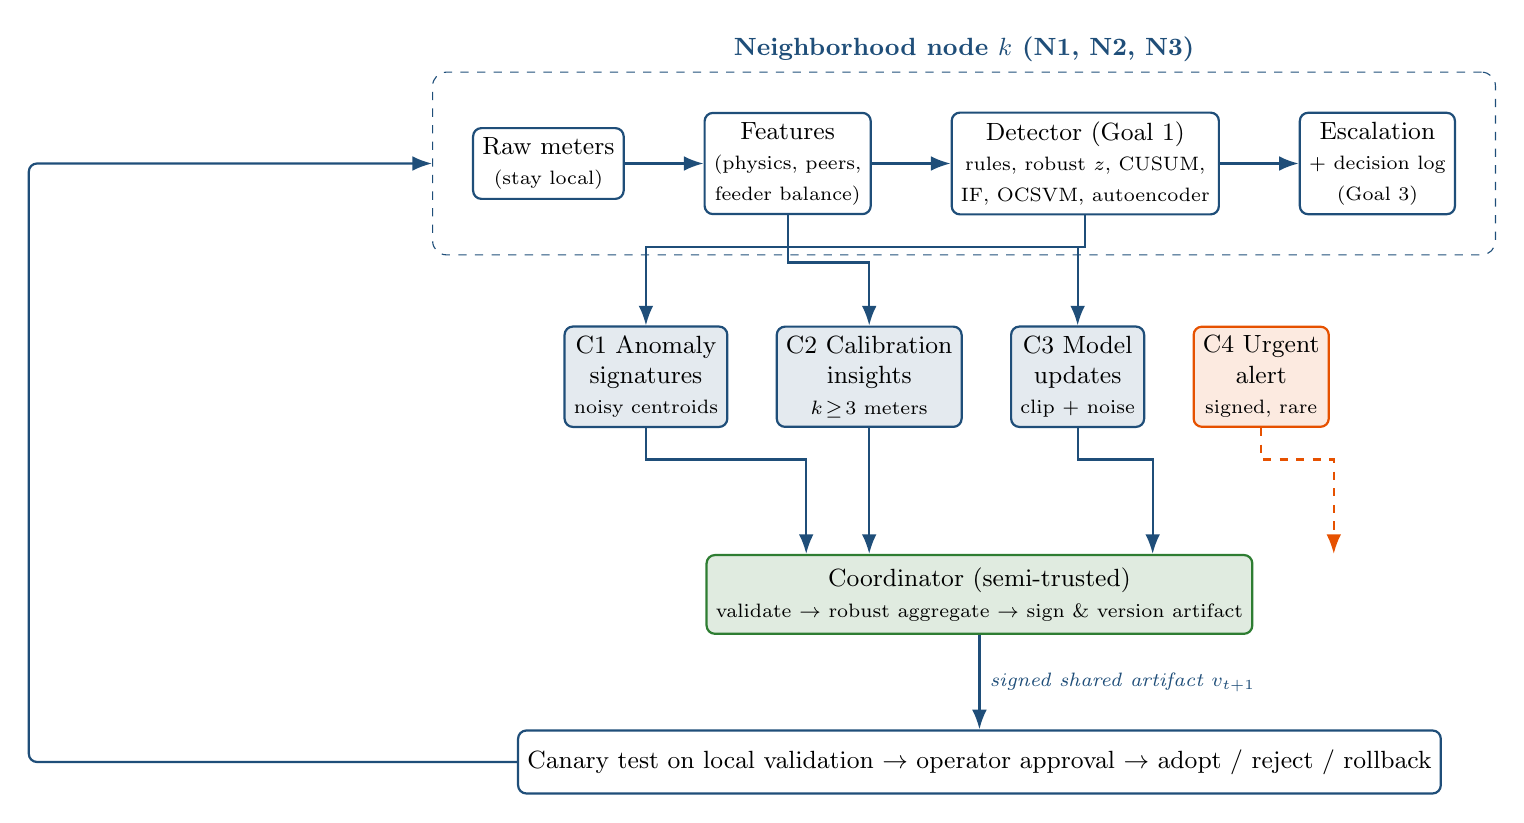
\begin{tikzpicture}[
  node distance=6mm and 10mm,
  box/.style={rectangle,rounded corners=3pt,draw=emblue,fill=emgrey,thick,align=center,minimum height=8mm,font=\small},
  local/.style={box,fill=white},
  chan/.style={box,fill=emblue!12},
  coord/.style={box,fill=emgreen!15,draw=emgreen,minimum height=10mm},
  arr/.style={-{Latex[length=2.5mm]},thick,emblue},
  warn/.style={-{Latex[length=2.5mm]},thick,emorange,dashed},
  lbl/.style={font=\scriptsize\itshape,emblue}]
% node stack
\node[local] (data) {Raw meters\\\scriptsize (stay local)};
\node[local,right=of data] (feat) {Features\\\scriptsize (physics, peers,\\\scriptsize feeder balance)};
\node[local,right=of feat] (det) {Detector (Goal 1)\\\scriptsize rules, robust $z$, CUSUM,\\\scriptsize IF, OCSVM, autoencoder};
\node[local,right=of det] (esc) {Escalation\\\scriptsize + decision log\\\scriptsize (Goal 3)};
\draw[arr] (data)--(feat); \draw[arr] (feat)--(det); \draw[arr] (det)--(esc);
\begin{scope}[on background layer]
 \node[draw=emblue,dashed,rounded corners=5pt,fit=(data)(feat)(det)(esc),inner sep=5mm,
       label={[font=\small\bfseries,emblue]above:Neighborhood node $k$ (N1, N2, N3)}] (nodebox) {};
\end{scope}
% channels
\node[chan,below=14mm of feat,xshift=-18mm] (c1) {C1 Anomaly\\ signatures\\\scriptsize noisy centroids};
\node[chan,right=6mm of c1] (c2) {C2 Calibration\\ insights\\\scriptsize $k\!\ge\!3$ meters};
\node[chan,right=6mm of c2] (c3) {C3 Model\\ updates\\\scriptsize clip + noise};
\node[chan,right=6mm of c3,draw=emorange,fill=emorange!12] (c4) {C4 Urgent\\ alert\\\scriptsize signed, rare};
\draw[arr] (det.south)--++(0,-4mm)-|(c1.north);
\draw[arr] (det.south)--++(0,-4mm)-|(c3.north);
\draw[arr] (feat.south)--++(0,-6mm)-|(c2.north);
% coordinator
\node[coord,below=16mm of c2,xshift=14mm] (co) {Coordinator (semi-trusted)\\\scriptsize validate $\to$ robust aggregate $\to$ sign \& version artifact};
\draw[arr] (c1.south)--++(0,-4mm)-|([xshift=-22mm]co.north);
\draw[arr] (c2.south)--(c2.south|-co.north);
\draw[arr] (c3.south)--++(0,-4mm)-|([xshift=22mm]co.north);
\draw[warn] (c4.south)--++(0,-4mm)-|([xshift=45mm]co.north);
% return
\node[local,below=12mm of co] (canary) {Canary test on local validation $\to$ operator approval $\to$ adopt / reject / rollback};
\draw[arr] (co)--node[lbl,right]{signed shared artifact $v_{t+1}$}(canary);
\draw[arr,rounded corners=3pt] (canary.west)--++(-62mm,0)|-(nodebox.west);
\end{tikzpicture}}
\caption{Noosphere architecture. Raw data and decisions stay inside the node; three protected channels and one urgent-alert path reach a coordinator, whose output is only adopted after a local canary test and human approval.}
\label{fig:arch}
\end{figure}

\subsection{What is shared, what stays local, and why}

\begin{table}[H]
\centering\small
\caption{Sharing contract. Each row answers the challenge's three questions: what, what stays local, why.}
\label{tab:sharing}
\begin{tabularx}{\textwidth}{@{}p{2.1cm} Y Y Y@{}}
\toprule\hdr
Channel & Shared artifact & Safeguards & Why it helps \\
\midrule
\textbf{C1} Anomaly patterns & Per-node centroids of ``trusted'' and ``untrusted'' records in a robustly standardised feature space (Eq.~\ref{eq:protocol-preprocessing}); optional per-\emph{family} centroids when $\ge n_{\min}$ events exist: physical bypass and data-only FDI (Goal~2 verdict \code{SUSPICIOUS\_DATA}), sensor drift and corruption (\code{METER\_FAULT}) & Feature clipping, Gaussian noise on released centroids, coordinate-wise median across nodes, count bucketing & Lets a node recognise an attack family it has seen too rarely to learn, without exchanging any time series \\
\addlinespace
\textbf{C2} Calibration insights & Median of $\log\!\big(E/(V\,I\,\mathrm{PF}\,\Delta t/1000)\big)$ per \emph{meter model} on clean, non-exporting readings, with sample size bucket & Release a model only if $\ge 3$ meters contribute; medians only; no meter IDs & Separates a model-wide calibration bias (firmware, batch) from a single faulty meter \\
\addlinespace
\textbf{C3} Model updates & Clipped, noised updates to a shared logistic-regression screening model & Update-norm clipping $C$, Gaussian noise $\sigma$, robust aggregation, secure aggregation (deployment) & Nodes with few rare events borrow strength from others; the shared model supports, never replaces, the local detectors of Goal~1 \\
\addlinespace
\textbf{C4} Urgent alert & Signed ``attack fingerprint'': subtype family, feature-residual profile, affected meter-model, severity & Human-confirmed at the source node; rate-limited; expires; receivers treat it as a \emph{prior}, not a verdict & Days-to-hours propagation of a confirmed coordinated attack \\
\bottomrule
\end{tabularx}
\end{table}

\paragraph{Stays local (never leaves the node):} raw readings and timestamps; meter, customer and feeder identifiers; coordinates and dwelling data; per-meter reference values and the local median/MAD scaling statistics; per-record features, verdicts and SHAP explanations; operator notes and overrides; full decision logs; local detector models. \emph{Reason:} half-hourly smart-meter traces reveal occupancy, sleep and appliance use~\cite{hart1992,molina2010}; explanations and logs are accountability records that belong to the operator that made the decision.

\subsection{Protocol}
\label{subsec:protocol}

The protocol defines how independent neighborhood nodes prepare local
information, share privacy-aware summaries or model updates, and evaluate
the knowledge received from the coordinator. Raw meter readings and
record-level decisions remain local. The protocol distinguishes four
sharing channels: anomaly signatures (C1), calibration insights (C2),
federated model updates (C3), and urgent alerts (C4). C1--C3 are regular
knowledge-sharing mechanisms, whereas C4 is a separate, rare alert path.

\subsubsection{Protocol overview}

Figure~\ref{fig:protocol-pipeline} presents the complete protocol, from
local data preparation to the local acceptance or rejection of a shared
model. The multi-node communication and secure aggregation components
are documented design requirements; the figure describes the proposed
architecture rather than claiming that the complete distributed system
has been deployed.

\begin{figure}[H]
\centering
\resizebox{\textwidth}{!}{%
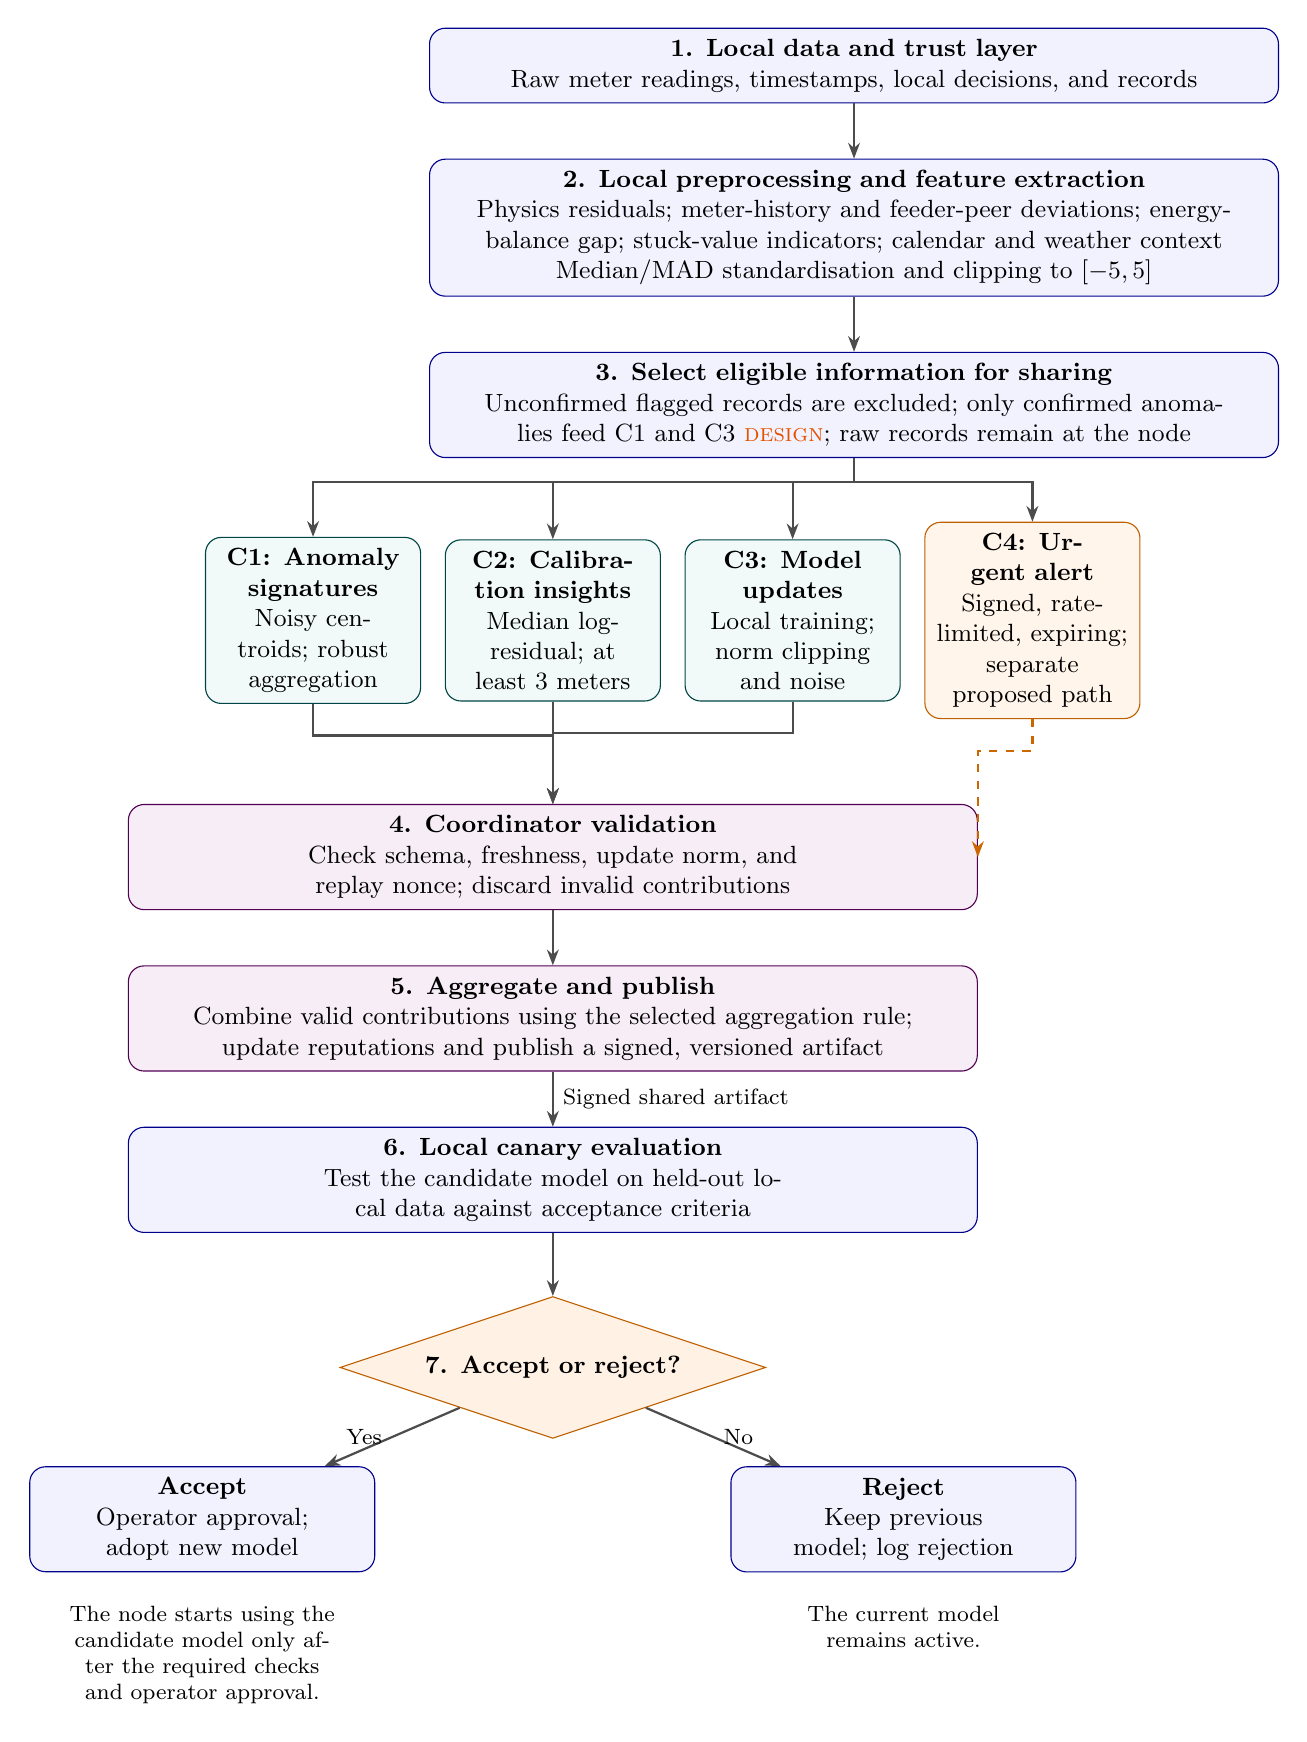
\begin{tikzpicture}[
    font=\small,
    node distance=7mm,
    process/.style={
        rectangle, rounded corners=2mm,
        draw=blue!55!black, fill=blue!5,
        text width=10.5cm, align=center,
        minimum height=9mm, inner sep=4pt
    },
    channel/.style={
        rectangle, rounded corners=2mm,
        draw=teal!55!black, fill=teal!5,
        text width=2.45cm, align=center,
        minimum height=16mm, inner sep=4pt
    },
    coordinator/.style={
        rectangle, rounded corners=2mm,
        draw=violet!65!black, fill=violet!7,
        text width=10.5cm, align=center,
        minimum height=12mm, inner sep=4pt
    },
    decision/.style={
        diamond, aspect=3.0,
        draw=orange!75!black, fill=orange!10,
        text width=4.0cm, align=center,
        inner sep=2pt
    },
    arr/.style={-{Stealth[length=2mm]}, thick, draw=black!70},
    note/.style={font=\footnotesize, align=center}
]

\node[process] (local) {
    \textbf{1. Local data and trust layer}\\
    Raw meter readings, timestamps, local decisions, and records
};

\node[process, below=of local] (prep) {
    \textbf{2. Local preprocessing and feature extraction}\\
    Physics residuals; meter-history and feeder-peer deviations;
    energy-balance gap; stuck-value indicators; calendar and weather context\\
    Median/MAD standardisation and clipping to $[-5,5]$
};

\node[process, below=of prep] (select) {
    \textbf{3. Select eligible information for sharing}\\
    Unconfirmed flagged records are excluded; only confirmed anomalies
    feed C1 and C3 \design{}; raw records remain at the node
};

\node[channel, below left=10mm and 1mm of select] (c1) {
    \textbf{C1: Anomaly signatures}\\
    Noisy centroids; robust aggregation
};

\node[channel, right=3mm of c1] (c2) {
    \textbf{C2: Calibration insights}\\
    Median log-residual; at least 3 meters
};

\node[channel, right=3mm of c2] (c3) {
    \textbf{C3: Model updates}\\
    Local training; norm clipping and noise
};

\node[channel, right=3mm of c3, draw=orange!75!black,
      fill=orange!8] (c4) {
    \textbf{C4: Urgent alert}\\
    Signed, rate-limited, expiring; separate proposed path
};

\node[coordinator, below=13mm of c2] (validate) {
    \textbf{4. Coordinator validation}\\
    Check schema, freshness, update norm, and replay nonce;
    discard invalid contributions
};

\node[coordinator, below=of validate] (aggregate) {
    \textbf{5. Aggregate and publish}\\
    Combine valid contributions using the selected aggregation rule;
    update reputations and publish a signed, versioned artifact
};

\node[process, below=of aggregate] (test) {
    \textbf{6. Local canary evaluation}\\
    Test the candidate model on held-out local data against acceptance criteria
};

\node[decision, below=of test, yshift=-1mm] (decision) {
    \textbf{7. Accept or reject?}
};

\node[process, below left=8mm and 9mm of decision,
      text width=4.1cm, minimum height=9mm] (accept) {
    \textbf{Accept}\\
    Operator approval; adopt new model
};

\node[process, below right=8mm and 9mm of decision,
      text width=4.1cm, minimum height=9mm] (reject) {
    \textbf{Reject}\\
    Keep previous model; log rejection
};

\draw[arr] (local) -- (prep);
\draw[arr] (prep) -- (select);
\draw[arr] (select.south) -- ++(0,-3mm) -| (c1.north);
\draw[arr] (select.south) -- ++(0,-3mm) -| (c2.north);
\draw[arr] (select.south) -- ++(0,-3mm) -| (c3.north);
\draw[arr] (select.south) -- ++(0,-3mm) -| (c4.north);

\draw[arr] (c1.south) -- ++(0,-4mm) -| (validate.north);
\draw[arr] (c2.south) -- (validate.north);
\draw[arr] (c3.south) -- ++(0,-4mm) -| (validate.north);
\draw[arr, dashed, draw=orange!80!black]
    (c4.south) -- ++(0,-4mm) -| (validate.east);

\draw[arr] (validate) -- (aggregate);
\draw[arr] (aggregate) -- node[right, note]
    {Signed shared artifact} (test);
\draw[arr] (test) -- (decision);
\draw[arr] (decision) -- node[left, note] {Yes} (accept);
\draw[arr] (decision) -- node[right, note] {No} (reject);

\node[note, below=3mm of accept, text width=4.2cm] {
    The node starts using the candidate model only after the required checks
    and operator approval.
};

\node[note, below=3mm of reject, text width=4.2cm] {
    The current model remains active.
};

\end{tikzpicture}%
}
\caption{Proposed shared-learning protocol. Raw readings and
record-level decisions remain local. C1--C3 carry regular shared
information; C4 is a separate proposed urgent-alert path. A shared
model is adopted only after local evaluation and operator approval.}
\label{fig:protocol-pipeline}
\end{figure}

\subsubsection{Step 1: Local preprocessing and feature extraction}

Each node processes its own meter data and constructs a feature vector
describing possible anomalies. The features combine:
\begin{itemize}
    \item physical consistency residuals between measured energy
    $E$ and the estimate $VI\,\mathrm{PF}\,\Delta t$;
    \item deviations from the meter's own historical behaviour;
    \item deviations from peer meters on the same feeder;
    \item the feeder energy-balance gap;
    \item indicators of stuck or repeated values;
    \item calendar and weather context.
\end{itemize}

Since feature scales and distributions may differ between nodes, each
node standardises feature $j$ using its own median and median absolute
deviation (MAD), and clips the result to a bounded interval:
\begin{equation}
z_{ij} =
\operatorname{clip}\!\left(
\frac{x_{ij}-\operatorname{med}_j}
     {1.4826\,\mathrm{MAD}_j},
-c,c
\right),
\qquad c=5.
\label{eq:protocol-preprocessing}
\end{equation}

Here, $x_{ij}$ is feature $j$ for record $i$;
$\operatorname{med}_j$ is the local median of feature $j$;
$\mathrm{MAD}_j$ is its median absolute deviation; and
$\operatorname{clip}(u,-c,c)$ restricts $u$ to the interval
$[-c,c]$. The factor $1.4826$ is a conventional scaling factor for
the MAD. The operation limits the influence of extreme feature values
on subsequent shared statistics.

Two kinds of local records are kept apart \design{}. Records that the
local trust layer has flagged but no one has confirmed are excluded from
everything that is shared, so an unverified anomaly can neither distort
the shared picture of normal behaviour nor be presented as an attack.
Records whose cause is confirmed (by an operator, or in the prototype by
the dataset labels \code{gt\_*}) are the \emph{only} anomalies used for
the ``untrusted'' and family centroids of C1 and for the screening model
of C3. This is a documented design rule and should not be interpreted as
proof that the complete multi-node exclusion mechanism has been deployed.

\subsubsection{Step 2: Prepare the information to be shared}

After local preprocessing, a node prepares the relevant artifact for
the selected sharing channel. The four channels serve different
purposes and must not be treated as interchangeable.

\paragraph{C1: Anomaly signatures.}

C1 shares compact representations of anomaly patterns, using centroids
of trusted and untrusted records in the standardised feature space.
When enough examples are available, centroids may also be maintained
for anomaly families such as physical bypass, data-only false data
injection (FDI), and sensor drift.

Before release, centroids use feature clipping and Gaussian noise;
the coordinator combines the received summaries using coordinate-wise
medians. Count bucketing is also specified as a safeguard. This allows
nodes to learn from patterns observed elsewhere without exchanging
individual meter time series.

\paragraph{C2: Calibration insights.}

C2 shares a robust summary of the calibration behaviour of a meter
model. For node $k$ and meter model $m$, the summary is released only
when at least three meters of that model are available locally,
$n_{k,m}\geq 3$:
\begin{equation}
\widetilde r_{k,m}
=
\operatorname{med}_{i\in m}
\operatorname{med}_{t}
\log\!\left(
\frac{E_{it}}
{V_{it} I_{it}\,\mathrm{PF}_{it}\,\Delta t/1000}
\right).
\label{eq:protocol-calibration-local}
\end{equation}

Here, $E_{it}$ is the measured energy for meter $i$ at time $t$;
$V_{it}$ is voltage; $I_{it}$ is current; $\mathrm{PF}_{it}$ is
power factor; and $\Delta t$ is the measurement interval (0.5~h; the
factor 1000 converts W$\cdot$h to kWh). Only clean readings with
$V>0$, no PV export and $E>0$ are used: while a home exports, its
imported energy is 0 and the logarithm is undefined. The inner median
summarises the time-dependent residual for each meter, while the outer
median summarises the meters belonging to model $m$.

The coordinator then takes the median of the summaries received from
eligible nodes:
\begin{equation}
\widetilde r_m
=
\operatorname{med}_{k}\widetilde r_{k,m}.
\label{eq:protocol-calibration-global}
\end{equation}

A value consistently far from zero across several nodes may indicate
a systematic bias associated with that meter model. A deviation
observed for only one meter is more consistent with an individual
meter fault. This is a diagnostic indication, not by itself proof of
the cause.

\emph{On our dataset C2 is a negative control.} The three meter models
differ only by communication technology (GPRS, NB-IoT, PLC), all meters
have accuracy class~1.0, and no model-wide bias was injected. Computed
on the clean data, $\widetilde r_{k,m}$ lies within $\pm0.0002$ (i.e.\
$\pm0.02\%$) for every node and model, so any larger value would be a
false alarm. With the $n_{k,m}\ge3$ rule, the PLC model (5 meters in N1,
none in N2, 2 in N3) is released by N1 only, so its ``median across
nodes'' rests on a single node. A positive test is planned
(Section~\ref{sec:eval}): a $+3\%$ gain is injected on all NB-IoT meters
\emph{inside the experiment code}, leaving the dataset unchanged; C2
must report it, while a single biased meter (\code{bias\_step}) must not
move the model-level value.

\paragraph{C3: Federated model updates.}

C3 allows nodes to contribute to a shared screening model without
transferring their local training records. At round $t$, node $k$
trains the current model $w_t$ on its local dataset $\mathcal D_k$.
The resulting update is
\begin{equation}
\Delta_k
=
\mathrm{LocalTrain}(w_t;\mathcal D_k)-w_t.
\label{eq:protocol-local-update}
\end{equation}

The update $\Delta_k$ represents the change produced by local training.
It is not the raw dataset and does not need to contain individual
meter readings.

\paragraph{C4: Urgent alerts.}

C4 is a separate proposed path for rare, urgent information. An alert
may contain a signed attack fingerprint describing the subtype family,
feature-residual profile, affected meter model, and severity. The
design requires confirmation by a human operator at the source,
rate limiting, and expiration. Receiving nodes should treat the alert
as a prior indication to investigate, not as a definitive verdict.
The full distributed alert path remains a design requirement.

The dataset contains a ready-made case. A \code{coordinated\_fdi}
attack (three meters of one feeder falsified together) hits N3 from
1 to 28~July 2025 and N1 from 14~October 2025. Once N3's operator
confirms the July attack, its fingerprint reaches N1 three months
before N1's own attack. Because Goal~1's physics rule already flags
data-only injection in N1 from the first day, the expected benefit of
the alert is not earlier detection but a faster and more confident
diagnosis: the receiving node can name a confirmed attack family
instead of an unexplained anomaly.

\subsubsection{Step 3: Protect model updates before sharing}

Before a C3 update is shared, the node clips its Euclidean norm and
adds Gaussian noise:
\begin{equation}
\widetilde{\Delta}_k
=
\Delta_k
\min\!\left(1,\frac{C}{\|\Delta_k\|_2}\right)
+
\mathcal N\!\left(
0,\frac{\sigma^2 C^2}{K}I
\right).
\label{eq:protocol-protected-update}
\end{equation}

The symbols have the following meanings:
\begin{itemize}
    \item $C$ is the maximum allowed update norm;
    \item $\|\Delta_k\|_2$ is the Euclidean norm of the local update;
    \item $\sigma$ is the noise multiplier;
    \item $K$ is the number of participating nodes;
    \item $I$ is the identity matrix;
    \item $\mathcal N(0,\frac{\sigma^2 C^2}{K}I)$ is the
    zero-mean Gaussian noise distribution used by the design.
\end{itemize}

If the update norm is no greater than $C$, the clipping factor is
one. If it exceeds $C$, the factor reduces the update until its norm
is $C$. Gaussian noise is then added as a privacy safeguard.

Clipping limits the influence of a single large update, while noise
is intended to reduce the information revealed by the shared update.
However, clipping and adding noise alone do not establish a formal
differential-privacy guarantee. Such a guarantee would require a
specified privacy analysis and accounting procedure.

\subsubsection{Step 4: Validate and aggregate contributions}

The coordinator first checks received contributions against the
announced protocol version and feature schema. It also checks
freshness, update norms, and replay nonces, discarding invalid
contributions. The protocol requires authenticated and encrypted
communication; secure aggregation remains a deployment design
requirement.

For valid C3 updates, the coordinator applies the selected aggregation
rule and updates the shared model:
\begin{equation}
w_{t+1}
=
w_t+
\operatorname{Agg}\!\left(
\widetilde{\Delta}_1,\ldots,
\widetilde{\Delta}_K
\right).
\label{eq:protocol-model-aggregation}
\end{equation}

Here, $\operatorname{Agg}$ is the aggregation function, and
$w_{t+1}$ is the candidate shared model for the next round. Three
aggregation rules are considered.

\paragraph{FedAvg.}

FedAvg takes the arithmetic mean of the protected updates:
\begin{equation}
\operatorname{Agg}_{\mathrm{FedAvg}}
=
\frac{1}{K}\sum_{k=1}^{K}
\widetilde{\Delta}_k.
\label{eq:protocol-fedavg}
\end{equation}

This provides a simple way to combine the contributions of all
participating nodes. However, an unusually large or malicious update
may still affect the average, which motivates robust alternatives.

\paragraph{Coordinate-wise median.}

The coordinator calculates the median separately for each model
coordinate $j$:
\begin{equation}
\left(\operatorname{Agg}_{\mathrm{med}}\right)_j
=
\operatorname{med}_{k}
\left(\widetilde{\Delta}_{k,j}\right).
\label{eq:protocol-coordinate-median}
\end{equation}

Compared with the mean, the coordinate-wise median is less sensitive
to extreme values in individual coordinates. Its robustness has
limits, especially when few nodes participate or several nodes
collude.

\paragraph{Reputation-weighted aggregation.}

The coordinator can also weight updates according to node reputation
and how far each update deviates from the median update:
\begin{equation}
\operatorname{Agg}_{\mathrm{rep}}
=
\sum_{k=1}^{K}\rho_k\widetilde{\Delta}_k,
\qquad
\rho_k\propto r_k\exp\!\left(-\frac{d_k}{\tau}\right),
\label{eq:protocol-reputation-aggregation}
\end{equation}
where
\begin{equation}
d_k =
1-\cos\!\left(
\widetilde{\Delta}_k,\,
\operatorname{med}_{k'}
\widetilde{\Delta}_{k'}
\right).
\label{eq:protocol-update-distance}
\end{equation}

In this expression, $r_k\in[0,1]$ is the reputation of node $k$,
$d_k$ measures the cosine distance between its update and the
coordinate-wise median update, and $\tau$ controls the effect of
that distance on the weight. The proportional weights are normalised
so that they sum to one. Reputation is designed to decrease after
rejected rounds and recover after accepted rounds.

The three aggregation rules are alternatives; they are not three
successive operations that must all be applied to the same update.
The choice of aggregation rule should be stated for each experiment
or deployment configuration.

For C1 anomaly centroids, the coordinator instead applies
coordinate-wise medians to the protected summaries. C2 calibration
summaries are combined using the median across eligible nodes, as
defined in Equation~\ref{eq:protocol-calibration-global}.

\subsubsection{Step 5: Publish the shared artifact}

After validation and aggregation, the coordinator publishes a signed,
versioned artifact containing the relevant shared result. The
coordinator announces the round identifier, protocol version,
feature-schema identifier, clipping and noise parameters $(c,C,\sigma)$,
and deadline. Nodes sign and submit their contributions through the
specified authenticated, encrypted channel.

Versioning allows nodes to identify which shared artifact they have
received. Signatures support integrity and origin verification, while
the validation checks help reject stale or malformed contributions.
These protections describe the intended protocol; they do not imply
that a complete secure multi-node transport and aggregation system
has been implemented.

\subsubsection{Step 6: Local canary evaluation and adoption}

A node does not automatically adopt a newly published model. It first
evaluates the candidate on held-out local canary data and checks the
following criteria:
\begin{itemize}
    \item ROC-AUC must not decrease beyond an allowed margin
    $\Delta_{\mathrm{AUC}}$;
    \item the false-positive rate must remain within the defined alarm
    budget;
    \item genuine \code{grid\_event} and \code{equipment\_failure}
    records must not be misclassified as data-quality problems;
    \item recall per attack \emph{family} (physical bypass, data-only
    FDI, sensor drift, corruption) must not decrease. Per-type recall
    cannot serve as a gate: each falsification type occurs at most once
    per node, so its recall can only be 0 or 1. A family gates adoption
    only where the node holds at least three events of it
    (Table~\ref{tab:canary}); otherwise its result is reported to the
    operator without blocking adoption.
\end{itemize}

\begin{table}[H]
\centering\small
\caption{Events per attack family and node, and whether the family can gate adoption ($\ge3$ events).}
\label{tab:canary}
\begin{tabular}{@{}l ccc@{}}
\toprule\hdr
Family & N1 & N2 & N3 \\
\midrule
Physical bypass & 3 (gate) & 2 & 2 \\
Data-only FDI & 5 (gate) & 2 & 3 (gate) \\
Sensor drift & 8 (gate) & 6 (gate) & 4 (gate) \\
Corruption & 25 (gate) & 14 (gate) & 14 (gate) \\
\bottomrule
\end{tabular}
\end{table}

The numerical thresholds for these criteria must be specified before
deployment. If the candidate passes the checks and receives the
required operator approval, the node adopts it. Otherwise, the node
retains its previous model and logs the rejection.

This local evaluation step limits the risk of adopting a shared model
that is less suitable for a particular neighborhood. It does not,
by itself, prove that the model is safe against every attack or that
the protocol improves detection performance.

\subsubsection{Implementation status and limitations}

The protocol combines local processing, protected information
sharing, robust aggregation, and local model evaluation. Its claims
must nevertheless be interpreted in light of the current
implementation scope:
\begin{itemize}
    \item The experimental data are synthetic; they are not real
    STEG meter readings.
    \item The complete multi-node sharing experiment has not been run.
    The current work does not establish a measured performance
    improvement from cross-node collaboration.
    \item Network transport, node authentication, and secure
    aggregation remain documented design requirements.
    \item The noise mechanisms described here should not be presented
    as a formal differential-privacy guarantee without a complete
    privacy analysis.
    \item Robust aggregation has limitations with a small number of
    participants. With only three nodes, for example, a coordinate-wise
    median cannot guarantee protection against coordinated malicious
    contributions.
\end{itemize}

Accordingly, this section specifies the proposed shared-learning
protocol and its safeguards. It distinguishes the mechanisms exercised
in the in-process prototype from the additional components required
for a secure, fully distributed deployment.
\subsection{Privacy: what is protected and what is not}

Layered protections, each with a distinct role: locality (no raw data), clipping (bounded influence), Gaussian noise (plausible deniability for individual contributions~\cite{dwork2014,abadi2016}), group suppression ($k\!\ge\!3$, in the spirit of $k$-anonymity~\cite{sweeney2002}, \emph{not} a DP guarantee) and secure aggregation so the coordinator sees only the sum~\cite{bonawitz2017}. Gradient-style updates can leak training data if sent in the clear~\cite{zhu2019}, which is why secure aggregation is part of the deployment design.

For FedAvg with all $K$ nodes participating in each of $R$ rounds, Gaussian noise multiplier $\sigma$ and clipping bound $C$, the R\'enyi-DP accounting of~\cite{mironov2017} gives
\begin{equation}
 \varepsilon(\delta)=\min_{\alpha>1}\Big[\tfrac{R\alpha}{2\sigma^2}+\tfrac{\ln(1/\delta)}{\alpha-1}\Big]
 =\tfrac{R}{2\sigma^2}+\sqrt{\tfrac{2R\ln(1/\delta)}{\sigma^2}},\qquad\delta=10^{-5}.
 \label{eq:dp}
\end{equation}
This assumes the summed noise (each node adds $\sigma^2C^2/K$) is observed only after secure aggregation. Table~\ref{tab:eps} evaluates Eq.~\eqref{eq:dp}; the values are computed from the formula, not measured on our data.

\begin{table}[H]
\centering\small
\caption{$\varepsilon$ at $\delta=10^{-5}$ from Eq.~\eqref{eq:dp} (node-level, FedAvg only).}
\label{tab:eps}
\begin{tabular}{@{}c rrr@{}}
\toprule\hdr
$\sigma$ & $R=10$ & $R=26$ & $R=52$ \\
\midrule
1 & 20.2 & 37.5 & 60.6 \\
2 & 8.8 & 15.5 & 23.8 \\
4 & 4.1 & 6.9 & 10.3 \\
8 & 2.0 & 3.3 & 4.7 \\
\bottomrule
\end{tabular}
\end{table}

\paragraph{Honest reading.} Even a weekly schedule ($R=52$) needs $\sigma\!\approx\!8$ for $\varepsilon<5$, and with $K=3$ that much noise will likely cost accuracy, which is exactly the privacy--utility trade-off the planned experiment will measure (Section~\ref{sec:eval}); no utility number is claimed in Phase~1. Eq.~\eqref{eq:dp} covers FedAvg only; it does not cover signatures, calibration summaries, class counts, participation metadata, or the median and reputation rules, which need their own analysis. Until secure aggregation and transport security are implemented and the accounting is reviewed, the system is \emph{privacy-aware}, not \emph{provably private}.

\subsection{Threat model and collective defence}

\begin{table}[H]
\centering\small
\caption{Threat--defence matrix and what remains uncovered.}
\label{tab:threats}
\begin{tabularx}{\textwidth}{@{}p{3.1cm} Y Y Y@{}}
\toprule\hdr
Threat & Example & Defence & Residual risk \\
\midrule
Honest-but-curious coordinator & Inspects each node's update/summary & Secure aggregation, noise, bucketed counts & Not implemented in the in-process prototype \\
Network eavesdropper / tamperer & Reads or alters artifacts in transit & TLS, signed and versioned artifacts & Key management out of scope \\
Curious peer node & Infers another node's behaviour from the shared model & Clipping, noise, $k\!\ge\!3$ suppression & No formal bound beyond Eq.~\eqref{eq:dp} \\
Poisoned update & Sign-flipped or oversized $\Delta$ & Norm clip, median / reputation, canary test & Tolerates at most 1 of 3 arbitrary outliers \\
Replay / stale update & Resends an old $\Delta$ & Round nonce, freshness check & --- \\
Backdoor / adaptive attack & Update crafted to blind the model to one subtype~\cite{bagdasaryan2020} & Canary per-family recall, human approval, rollback & Not proven robust; basic defences are known to be weak \\
False alert injection (C4) & Fake ``attack fingerprint'' to cause alarms or desensitise & Source-node human confirmation, signature, rate limit, expiry, prior-only use & Sybil nodes need controlled registration \\
Collusion / Sybil & Majority of nodes (or fake identities) collude & Controlled node registration, governance rules & \textbf{Not defended}: median fails if $\ge2$ of 3 collude \\
\bottomrule
\end{tabularx}
\end{table}

\paragraph{Over-trust and under-trust of shared knowledge.} The Goal~3 concern about operators applies to the network as well. \emph{Over-trust} (blindly adopting a shared model) is prevented by the canary test, per-family recall checks, human approval and rollback. \emph{Under-trust} (rejecting useful updates forever) is monitored: every rejection is logged with its reason and the shadow-model comparison, so a persistent pattern of rejected-but-beneficial updates is visible to reviewers. Shared outputs only adjust anomaly scores; they do not change the autonomy thresholds or trigger any action on the grid, and Goal~3's non-tunable routing rules (R0--R3) apply whatever is shared.



\subsection{Evaluation plan}
\label{sec:eval}

No experiment across nodes has been run yet, and no performance number for sharing is claimed. The planned evaluation, all on the existing dataset (no change to the data), is:
\begin{enumerate}
  \item \textbf{Splits.} A calendar split does not work: in N1, November--December contain no falsification and no sensor-bias event. Models are therefore evaluated by cross-validation with folds grouped by event (\code{gt\_event\_id}), as in Goals~1--2; results are reported per event, with intervals. The \code{gt\_*} columns are never model inputs.
  \item \textbf{Transfer to unseen attacks.} For every attack type that is missing in some node (Table~\ref{tab:pernode}), train on the nodes that have it and score its events while the receiving node's own data contain no example of it; compare local only, local + C1 centroids, and local + C3 (FedAvg vs.\ coordinate-wise median). Measure per-family recall at a fixed false-positive rate.
  \item \textbf{Privacy--utility.} Repeat the C3 run for $\sigma\in\{1,2,4,8\}$ and plot detection against the $\varepsilon$ of Table~\ref{tab:eps}.
  \item \textbf{Corrupted node.} One node sends sign-flipped or scaled updates; compare FedAvg, median and reputation-weighted aggregation, and check that the canary rejects the poisoned artifact.
  \item \textbf{C2.} Negative control on the clean data (all models $\approx0$), then the $+3\%$ NB-IoT injection done in code.
  \item \textbf{C4.} N3's July coordinated attack as a prior for N1 before 14~October: diagnosis time and confidence with and without the alert.
\end{enumerate}

\subsection{Limitations}

\begin{enumerate}
  \item All data and anomalies are synthetic; results may reflect the simulator and cannot establish real-grid performance. External validation (e.g.\ Low Carbon London, UCI) is needed.
  \item The three nodes come from one generator, so their heterogeneity understates that of independent real operators.
  \item With $K=3$, robust aggregation has almost no redundancy and strong DP is costly (Table~\ref{tab:eps}).
  \item The corrupted-node tests do not cover backdoors, collusion, adaptive attacks, Sybil identities or a compromised coordinator.
  \item The simulated evasion attack is a random-walk scaling, not the gradient-based attacks of the literature.
  \item Each falsification type occurs 2--3 times in the dataset and at most once per node, so per-type results are case studies; families are used for decisions, with wide uncertainty.
\end{enumerate}

\begin{thebibliography}{99}\small
\bibitem{hart1992} G.~W.~Hart, ``Nonintrusive appliance load monitoring,'' \emph{Proc.\ IEEE}, vol.~80, no.~12, 1992.
\bibitem{molina2010} A.~Molina-Markham et al., ``Private memoirs of a smart meter,'' \emph{ACM BuildSys}, 2010.
\bibitem{sweeney2002} L.~Sweeney, ``$k$-anonymity: a model for protecting privacy,'' \emph{Int.\ J.\ Uncertainty, Fuzziness and Knowledge-Based Systems}, 2002.
\bibitem{mcmahan2017} B.~McMahan et al., ``Communication-efficient learning of deep networks from decentralized data,'' \emph{AISTATS}, 2017.
\bibitem{yin2018} D.~Yin et al., ``Byzantine-robust distributed learning: towards optimal statistical rates,'' \emph{ICML}, 2018.
\bibitem{blanchard2017} P.~Blanchard et al., ``Machine learning with adversaries: Byzantine tolerant gradient descent,'' \emph{NeurIPS}, 2017.
\bibitem{fung2018} C.~Fung et al., ``Mitigating sybils in federated learning poisoning,'' arXiv:1808.04866, 2018.
\bibitem{bonawitz2017} K.~Bonawitz et al., ``Practical secure aggregation for privacy-preserving machine learning,'' \emph{ACM CCS}, 2017.
\bibitem{dwork2014} C.~Dwork and A.~Roth, ``The algorithmic foundations of differential privacy,'' \emph{Found.\ Trends Theor.\ Comput.\ Sci.}, 2014.
\bibitem{abadi2016} M.~Abadi et al., ``Deep learning with differential privacy,'' \emph{ACM CCS}, 2016.
\bibitem{mironov2017} I.~Mironov, ``R\'enyi differential privacy,'' \emph{IEEE CSF}, 2017.
\bibitem{zhu2019} L.~Zhu, Z.~Liu, S.~Han, ``Deep leakage from gradients,'' \emph{NeurIPS}, 2019.
\bibitem{bagdasaryan2020} E.~Bagdasaryan et al., ``How to backdoor federated learning,'' \emph{AISTATS}, 2020.
\end{thebibliography}

\end{document}